\documentclass[11pt,a4paper]{article}
%-------------------------------------------
%---Packages--------------------------------
%-------------------------------------------
\usepackage[utf8]{inputenc}
%\usepackage[T1]{fontenc}
%\usepackage{txfonts}
\usepackage{amsmath}
\usepackage{amsthm}
\usepackage{amsfonts}
\usepackage{array}
\usepackage{amssymb}
\usepackage{blindtext}
\usepackage{caption}
\usepackage{color}
\usepackage{csquotes}	    %
\usepackage{enumitem}	    %pour mieux bosser avec les listes. ajoute option label
\usepackage[yyyymmdd]{datetime}        %pour définir date custom
\usepackage{etaremune}
\usepackage{environ}
\usepackage{fancybox}
\usepackage{fancyhdr} 	    % Custom headers and footers
\usepackage{fancyref}
%\usepackage{float}
\usepackage{floatrow}       %float and floatrow can't be together...
\usepackage{gensymb}
\usepackage{graphicx}
\usepackage[colorlinks=true, linkcolor=purple, citecolor=cyan]{hyperref}
\usepackage{footnotebackref}
\usepackage{lipsum}
\usepackage{mathtools}
\usepackage{multicol}	    %gérer plusieurs colonnes
\usepackage{setspace}
\usepackage{subcaption}
\usepackage{todonotes}	    %Bonne gestion des TODOs
%TODO commenté pour tester l'utilité... à voir% \usepackage[tc]{titlepic}      %Permet de mettre une image en page de garde
\usepackage{tikz}	    % Pour outil de dessin puissant
\usepackage{ulem}	    %underline sur plusieurs lignes (avec \uline{})
\usepackage{vmargin} 	    %gestion des marges, avec dans l'ordre : gauche, haut, droit, bas, en-tête, entre en-tête et texte, bas de page, hauteur entre bas de page et texte
\usepackage{wrapfig}
\usepackage{xcolor}
\usepackage{xparse}                    %Pour utiliser NewDocumentCommand et des arguments 'mmooo'
%\usepackage{fullpage} 	    %supprime toutes les marges allouées aux notes, aussi en haut et en bas

%\ExplSyntaxOn
\pagestyle{fancyplain}	    %Makes all pages in the document conform to the custom headers and footers

%-------------------------------------------
%---Document Commands-----------------------
%---------------------------{----------------
\NewDocumentCommand{\framecolorbox}{oommm}
 {% #1 = width (optional)
  % #2 = inner alignment (optional)
  % #3 = frame color
  % #4 = background color
  % #5 = text
  \IfValueTF{#1}%
   {\IfValueTF{#2}%
    {\fcolorbox{#3}{#4}{\makebox[#1][#2]{#5}}}%
    {\fcolorbox{#3}{#4}{\makebox[#1]{#5}}}%
   }%
   {\fcolorbox{#3}{#4}{#5}}%
 }%
%------------------------------------------------
%------------------ENGLISH----------------------
%----------------------------------------------

\NewDocumentCommand{\epflTitle}{mO{Olivier Cloux}O{\today}O{Notes de Cours en}D<>{../../Common}}%Arguments : Matière, Auteur, Date, Titre du doc
{
\begin{titlepage}
    \vspace*{\fill}
    \begin{center}
        \normalfont \normalsize
        \textsc{Ecole Polytechnique Fédérale de Lausanne} \\ [25pt] % Your university, school and/or department name(s)
        \textsc{#4} %Titre du doc
        \\ [0.4 pt]
        \horrule{0.5pt} \\[0.4cm] % Thin top horizontal rule
        \huge #1 \\ % Matière
        \horrule{2pt} \\[0.5cm] % Thick bottom horizontal rule
        
\includegraphics[width=8cm]{#5/EPFL_logo}
        ~\\[0.5 cm]
        \small\textsc{#2}\\[0.4cm]
        \small\textsc{#3}\\
        ~\\
        ~\\
        
\includegraphics[scale=0.5]{#5/creativeCommons}
    \end{center}
    \vspace*{\fill}
\end{titlepage}
}


%-------------------------------------------
%-------------MATH NEW COMMANDS-------------
%-------------------------------------------
\newcommand{\somme}[2]{\ensuremath{\sum\limits_{#2}^{#1}}}
\newcommand{\produit}[2]{\ensuremath{\prod\limits_{#2}^{#1}}}
\newcommand{\limite}{\lim\limits_}
\newcommand{\llimite}[3]{\limite{\substack{#1 \\ #2}}\left(#3\right)}	%limites à deux condiitons
\newcommand{\et}{\mbox{ et }}
\newcommand{\deriv}[1]{\ensuremath{\, \mathrm d #1}}	%sigle dx, dt,dy... des dérivées/intégrales
%\newcommand{\fx}{\ensuremath{f'(\textbf{x}_0 + h}}
\newcommand{\ninf}{\ensuremath{n \to \infty}}	       %pour les limites : n tend vers l'infini
\newcommand{\xinf}{\ensuremath{x \to \infty}}	       %pour les limites : x tend vers l'infini
\newcommand{\infint}{\ensuremath{\int_{-\infty}^{\infty}}}
\newcommand{\xo}{\ensuremath{x \to 0}}									%x to 0
\newcommand{\no}{\ensuremath{n \to 0}}									%n zéro
\newcommand{\xx}{\ensuremath{x \to x}}									%x to x
\newcommand{\Xo}{\ensuremath{x_0}}										%x zéro
\newcommand{\X}{\ensuremath{\mathbf{X}} }
\newcommand{\A}{\ensuremath{\mathbf{A}} }
\newcommand{\R}{\ensuremath{\mathbb{R}} }								%ensemble de R
\newcommand{\rn}{\ensuremath{\mathbb{R}^n} } 							%ensemble de R de taille n
\newcommand{\Rm}{\ensuremath{\mathbb{R}^m} }  							%ensemble de R de taille m
\newcommand{\C}{\ensuremath{\mathbb{C}} }
\newcommand{\N}{\ensuremath{\mathbb{N}} }
\newcommand{\Z}{\ensuremath{\mathbb{Z}} }
\newcommand{\Q}{\ensuremath{\mathbb{Q}} }
\newcommand{\rtor}{\ensuremath{\R \to \R} }
\newcommand{\pour}{\mbox{ pour }}
\newcommand{\coss}[1]{\ensuremath{\cos\(#1\)}}						%cosinus avec des parenthèses de bonne taille (genre frac)
\newcommand{\sinn}[1]{\ensuremath{\sin\(#1\)}}					%sinus avec des parentèses de bonne taille (genre frac)
\newcommand{\txtfrac}[2]{\ensuremath{\frac{\text{#1}}{\text{#2}}}}		%Fractions composées de texte
\newcommand{\evalfrac}[3]{\ensuremath{\left.\frac{#1}{#2}\right|_{#3}}}
\renewcommand{\(}{\left(}												%Parenthèse gauche de taille adaptive
\renewcommand{\)}{\right)}
\newcommand{\longeq}{=\joinrel=}												%Parenthèse droite de taille adaptive


%-------------------------------------------------------
%------------------MISC NEW COMMANDS--------------------
%-------------------------------------------------------
\newcommand{\degre}{\ensuremath{^\circ}}
%\newdateformat{\eudate}{\THEYEAR-\twodigit{\THEMONTH}-\twodigit{\THEDAY}}



%-------------------------------------------------------
%------------------TEXT NEW COMMANDS--------------------
%-------------------------------------------------------
\newcommand{\ts}{\textsuperscript}
\newcommand{\evid}[1]{\textbf{\uline{#1}}}        %mise en évidence (gras + souligné)



%\newcommand{\Exemple}{\underline{Exemple}}
\newcommand{\Theoreme}{\underline{Théorème}}
\newcommand{\Remarque}{\underline{Remarque}}
\newcommand{\Definition}{\underline{Définition} }
\newcommand{\skinf}{\sum^{\infty}_{k=0}}
\newcommand{\combi}[2]{\ensuremath{\begin{pmatrix} #1 \\ #2 \end{pmatrix}}}	%combinaison parmi 1 de 2
\newcommand{\intx}[3]{\ensuremath{\int_{#1}^{#2} #3 \deriv{x}}}				%intégrale dx
\newcommand{\intt}[3]{\ensuremath{\int_{#1}^{#2} #3 \deriv{t}}}				%intégrale dy
\newcommand{\misenforme}{\begin{center} Mis en forme jusqu'ici\\ \line(1,0){400}\\ normalement juste, mais à améliorer depuis ici\end{center}}	%raccourci pour mise en forme
\newcommand*\circled[1]{\tikz[baseline=(char.base)]{
            \node[shape=circle,draw,inner sep=1pt] (char) {#1};}}			%pour entourer un chiffre
\newcommand{\horrule}[1]{\rule{\linewidth}{#1}} 				% Create horizontal rule command with 1 argument of height

\theoremstyle{definition}
\newtheorem{exemp}{Exemple}
\newtheorem{examp}{Example}


%-------------------------------------------
%---Environments----------------------------
%-------------------------------------------
\NewEnviron{boite}[1][0.9]{%
	\begin{center}
		\framecolorbox{red}{white}{%
			\begin{minipage}{#1\textwidth}
 	 			\BODY
			\end{minipage}
		}
	\end{center}
}
\NewEnviron{blackbox}[1][0.9]{%
	\begin{center}
		\framecolorbox{black}{white}{%
			\begin{minipage}{#1\textwidth}
 	 			\BODY
			\end{minipage}
		}
	\end{center}
}
\NewEnviron{exemple}[1][0.8]{%
    \begin{center}
        \framecolorbox{white}{gray!20}{%
            \begin{minipage}{#1\textwidth}
                \begin{exemp}
                    \BODY
                \end{exemp}
            \end{minipage}
        }
    \end{center}
}
\NewEnviron{suiteExemple}[1][0.8]{%
    \begin{center}
        \framecolorbox{white}{gray!20}{%
            \begin{minipage}{#1\textwidth}
                \BODY
            \end{minipage}
        }
    \end{center}
}
\NewEnviron{colExemple}[1][0.8]{%
    \begin{center}
        \framecolorbox{white}{gray!20}{%
            \begin{minipage}{#1\columnwidth}
                \begin{exemp}
                    \BODY
                \end{exemp}
            \end{minipage}
        }
    \end{center}
}
\NewEnviron{example}[1][0.8]{%
    \begin{center}
        \framecolorbox{white}{gray!20}{%
            \begin{minipage}{#1\textwidth}
                \begin{examp}
                    \BODY
                \end{examp}
            \end{minipage}
	}
    \end{center}
}
\NewEnviron{systeq}[1][l]{
			\begin{center}
				$\left\{\begin{array}{#1}
					\BODY
				\end{array}\right.$
			\end{center}
 }





%-------------------------------------------
%---General settings-----------------------
%-------------------------------------------
\renewcommand{\headrulewidth}{1pt}										%ligne au haut de chaque page
\renewcommand{\footrulewidth}{1pt}										%ligne au pied de chaque page
\setstretch{1.6}
\author{Olivier Cloux}

%%%%%%%%%%%%%%%%%%%%%%%%%%%%%%%%%%%%%%%%%%%%
%%TODO : Supprimer quand plus de todo %%%%%%
\marginparwidth = 75pt
\textwidth = 400pt
%%%%%%%%%%%%%%%%%%%%%%%%%%%%%%%%%%%%%%%%%%%%
\usepackage{titlesec}
\numberwithin{equation}{section}
\newtheorem{defin}{Definition}
\NewEnviron{definition}[1][0.9]{%
    \begin{center}
        \framecolorbox{black}{white}{%
            \begin{minipage}{#1\textwidth}
                \begin{defin}
                    \BODY
                \end{defin}
            \end{minipage}
	}
    \end{center}
}
\titleformat{\section}{\Large\bfseries}{}{0pt}{Lecture \thesection:\ }
\begin{document}
\epflTitle{Signal Processing for Communications}[Olivier Cloux][Spring 2017]
\tableofcontents

\section{Introduction}
The first question we need to ask, is \textit{What is a signal ?} For our interest, it is a description of the evolution of a physical phenomenon.
\begin{example}
    Temperature is a signal, as well as pressure, magnetic deviation, grey level on paper (for a photograph, thus this is a two dimensional signal),...
\end{example}

\textbf{Analysing} a signal is \textit{understanding} the information carried by the signal, while on the opposite, \textbf{synthesising} a signal is \textit{creating} a signal that contains such information.
Concerning communications, we have a great parallel : \textbf{reception} is the \textit{analysis} of an incoming signal and \textbf{transmission} is the \textit{synthesis} of an outgoing signal.

We can model a signal using classical electric circuits (with resistors, concentrators,..) but this model is limited. Modelling a person talking in a microphone with a circuits would require enormous work. To counter that, we created the \textbf{discrete model}. This model ``simplifies'' the system by discretizing the time axis, and the value axis. 

\begin{example}
    Instead of looking at the temperature continuously, it is much simpler to measure it at regular intervals.
\end{example}
But discretizing temperatures is appealing, because is does not change much. A cold day is a cold day. But when discretizing a voice, we need to change our model, especially time. What is time ? Philosophers have wondered so for many years. We remember the dichotomy paradox (an arrow going from A to B will first go through half, then quarter, the eighth, and so on infinitely, meaning the arrow never reaches B) ; this paradox is an example of why we need to be consistent mathematically. 

When computing a cannonball shooting, we can either measure the points or use calculus to find trajectory. This easy. But given any sample of data, finding the average with ``idealisation'' of the data is hard, as we need to find the perfectly fitting function and then compute the integral. Quite simpler to sum the points and divide by the number of points ! This is what signal processing is about.

But we can go back and forth between a signal and its sampled version with the following formula :\todo{rajouter}
\begin{boite}
    The Sampling Theorem :
    \begin{equation}
        \begin{array}{ll}
            x(t) &= \somme{n=-\infty}{\infty}
        \end{array}
    \end{equation}
\end{boite}
What this theorem says, is that once we are sampled, we can apply this sinc function at each points to obtain a lot of sin-like functions. And summing them will give us our original signal back.

\section{Discrete-Time Signals}
\subsection{Discrete-Time signals}
Discrete time signals come back long ago. For example, Egyptians used to keep record of floods of the Nile on tablets. We have a long history of signals, natural or not (in economy, population, astronomy,...). 

More Formally : 
\begin{boite}
    A discrete signal is a sequence of \textbf{complex} numbers.
    \begin{itemize}
        \item One dimension
        \item We note it $x[n]$
        \item Two-sided sequence : $x : \Z \to \C$
        \item $n$ is a-dimensional ``time''
        \item analysis : Periodic measurement
        \item synthesis : stream of generated samples
    \end{itemize}
\end{boite}
Our first and most simple signal : the delta signal. Value 0 everywhere but at 0
\begin{figure}
    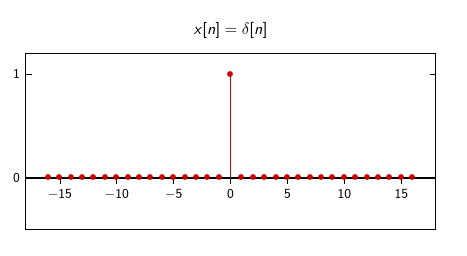
\includegraphics[scale=0.6]{images/delta}
\end{figure}
This signal is very useful, for example when synchronizing audio and video in a film : the clap is kind of a ``delta'' signal for audio.

Next simple signal : the \textit{unit step} :
\begin{figure}
    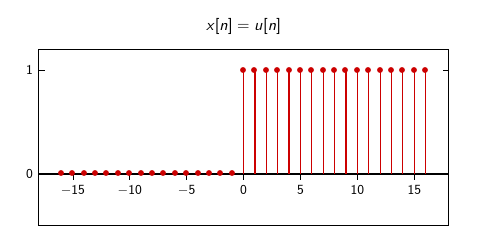
\includegraphics[scale=0.6]{images/unit_signal}
\end{figure}
and the \textit{exponential decay}
\begin{figure}
    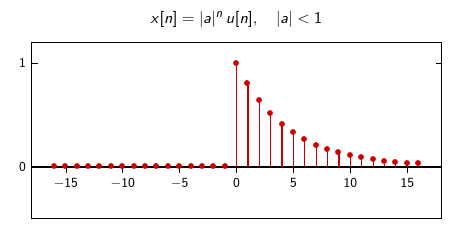
\includegraphics[scale=0.6]{images/expo_decay}
\end{figure}
\begin{example}
    Good examples of exponential decay : a coffee is going cold with exponential decay. Also how a capacitor discharges.
\end{example}x
For the well-known \textit{sinusoid} (discrete of course) we need the frequency and \todo{second ?}
\subsubsection{Signal classes}
We will consider 4 classes of signal : 
\begin{itemize}
    \item finite-length, used for practicality, the only visible signals
    \item infinite-length, used for theorems and proofs
    \item periodic, kind of an intermediate
    \item finite-support, also an intermediate
\end{itemize}
\subsubsection{Finite length}
Sequence notation :
\begin{equation}
    x[n],\ n=0,1,\ldots,N-1
\end{equation}
In a vector notation : 
\begin{equation}
    \mathbf{x} = [x_0x_1...x_{N-1}]^T
\end{equation}
\subsubsection{Infinite-length}
Sequence notation : 
\begin{equation}
    x[n],\ n\in \Z
\end{equation}
It is only an abstraction

\subsubsection{Periodic}
N-periodic sequence : 
\begin{equation}
    \tilde{x}[n] = \tilde{x}[n+kN],\ n,k,N \in \Z
\end{equation}
\todo{def}
\subsubsection{Finite-support}
\todo{def}
\subsection{Elementary signal operations}
Our main operators will be :
\begin{itemize}
    \item scaling
        \[y[n] = \alpha x[n]\]
    \item sum
        \[y[n] = x[n] + z[n]\]
    \item product
        \[y[n] = x[n] \cdot z[n]\]
    \item shift by k (delay)
        \[y[n] = x[n-k]\]
\end{itemize}
The shift for a finite-length signal can be tricky. There are two ways of doing so : either we add zeros behind the shifted sequence (1,2,3,4,5) becomes (0,1,2,3,4) or we consider it periodic and the shift is circular (1,2,3,4,5) becomes (5,1,2,3,4).

It's now important to define the energy and the power of a signal : 
\begin{align}
    E_x = \somme{n=-\infty}{\infty}|x[n]|^2\\
    P_x = \limite{N\to\infty} \frac{1}{2N+1} \somme{n=-N}{N}|x[n]|^2
\end{align}
Clearly, periodic signals have an infinite energy and a power of 
\[P_{\tilde{x}} \equiv \somme{n=0}{N-1}|\tilde{x}[n]|^2\]

\subsection{The Karplus-Strong Algorithm}

\section{Signal Processing and Vector spaces}
As we saw, signal is the description of the evolution of a physical phenomenon (as an RC circuit for example). Thus, we don't model the situation but use an ordered sequence of values. Then, our model for this kind of situations is $\C^N$. $N$ can very well be infinite. We will need more than just a vector space, we will use a Hilbert space.
\subsection{Vector spaces}
$\R^2$ and $\R^3$ are very familiar to us, they are Euclidean space used for everyday geometry. $\R^N$ and $\C^N$ are less familiar, as they require formal linear algebra because we can't construct a mental image. But even less familiars : $\ell_2(\Z)$ is the space of square-summable infinite sequence, and $L_2([a,b])$ is the space of square-integrable functions over an interval. We use vector spaces for easier maths and simplified framework.

\begin{definition}
    A vector space needs : the set of vectors $V$ and a set of scalars (say $\C$).
    
    We need at least to be able to resize vectors and combine vectors together. We define them as we want, but the vector space needs to fulfil the basic properties
\end{definition}
\todo{ajouter properties}
\begin{example}
    $\R^N$ is indeed a vector space, as resize and combination is well defined and fulfils the properties above.
\end{example}
But now we need something to measure and compare vectors : let's use the \textbf{inner product} (or \textbf{dot product}).

\begin{definition}
    \begin{equation}
        <\cdot,\cdot> : V \times V \to \C
    \end{equation}
    Measure of similarity between vectors. If the inner product is 0, then they are orthogonal. We could define it as we want, but still have a list of properties that need to be fulfilled. 
\end{definition}

\subsubsection{Inner product for signals}
\begin{equation}
    <\mathbf{x,y}> = \somme{N-1}{n=0} x^*[n]y[n]
\end{equation}
Careful, as with infinite signals, this sum may explode. Thus we require sequences to be \textit{square-summable} : $\sum |x[n]|^2 < \infty$
\subsection{Bases}
Can we find a set of vectors $\{\mathbf{w}^{(k)}\}$ so that we can write any vector as a linear combination of $\{\mathbf{w}^{(k)}\}$
\subsubsection{Basis expansion}
\begin{equation}
    \mathbf{x} = \somme{K-1}{k=0}\alpha_k \mathbf{w}^{(k)}
\end{equation}
But how do we find those ? Better use orthonormal bases !
\todo{missing}

\subsection{Hilbert space}
A vector space $H(V,\C)$, an inner product $V\times V \to \C$ and completeness. Completeness is : limiting operations must yield vector space elements.

\section{Introduction to Fourier Analysis}
Signals are often expressed as a linear combination of ``atomic'' time units, using Dirac :
\begin{equation}
    x[n] = \somme{N-1}{k=0}x[k]\delta[n-k]
\end{equation}
In vector notation : 
\begin{equation}
    \mathbf{x} = \somme{N-1}{k=0}x_k\mathbb{\delta}^{(k)}
\end{equation}
Fourier analysis is to express a signal as a combination of periodic oscillations. Fourier transform is a change of basis in the space of discrete-time signals. 
\end{document}